% ============================================================
% IEEE Transactions Conversion
% Scene-Adaptive Video Compression via DRL
% ============================================================
\documentclass[10pt,journal]{IEEEtran}

\usepackage{cite}
\usepackage{graphicx}
\usepackage{amsmath,amssymb,amsfonts}
\usepackage{booktabs}
\usepackage{url}
\usepackage[ruled,vlined,linesnumbered]{algorithm2e}
\usepackage{xcolor}
\usepackage{placeins}  % provides \FloatBarrier

\begin{document}

\title{Scene-Adaptive Video Compression Using Deep Reinforcement Learning for Safety-Critical Traffic Sign Detection}
\author{Anonymous Author(s)}

\maketitle

% ============================================================
% ABSTRACT
% ============================================================

\begin{abstract}
Deploying real-time traffic sign detection on bandwidth-constrained edge devices requires compression strategies that adapt to varying scene conditions without compromising the detection of safety-critical objects. Conventional video codecs (e.g., H.264/HEVC) optimize for human-perceived quality via rate-distortion trade-offs, which can suppress the high-frequency features that neural object detectors rely upon. Moreover, fixed compression ratios cannot accommodate the stochastic nature of traffic environments, where a sudden transition from a clear highway to a rain-obscured intersection demands an immediate shift in visual fidelity.

In this paper, we propose an end-to-end adaptive compression framework that integrates Snapshot Compressive Imaging (SCI), a YOLO11s object detector operating directly on compressed measurements, and a Deep Q-Network (DQN) agent that dynamically selects the temporal compression ratio. The agent observes a lightweight 7-dimensional state vector capturing motion, scene complexity, and detector confidence, and adjusts the compression ratio at each time step. A key novelty of our approach is a \emph{safety-aware reward function} that imposes a heavy penalty when the system fails to detect critical traffic signs (e.g., Stop, Yield) under adverse conditions. Evaluated on the CURE-TSD dataset across eight compression levels ($B \in \{6,8,10,12,14,16,18,20\}$), our adaptive policy achieves bandwidth savings of 90.6\% with 128.6 average detections per video, matching the detection performance of the optimal fixed baseline while adapting compression per-scene---reducing $B$ to 9.0 under noise (preserving safety) and increasing $B$ to 14.3 under rain (saving bandwidth).

\end{abstract}

\begin{IEEEkeywords}
Deep Reinforcement Learning, Snapshot Compressive Imaging, Adaptive Video Compression, Traffic Sign Detection, Edge Computing.
\end{IEEEkeywords}

% ============================================================
% 1. INTRODUCTION
% ============================================================

\section{Introduction}

The proliferation of autonomous vehicles (AVs) and intelligent transportation systems (ITS) has created an escalating demand for real-time video transmission over bandwidth-constrained wireless networks. A single 1080p camera operating at 30~FPS generates approximately 1.5~Gbps of raw data~\cite{sullivan2012hevc}, which far exceeds the uplink capacity of typical LTE or sub-6~GHz 5G deployments. Transmitting this data to cloud or edge servers for processing requires aggressive compression, yet the compression must preserve the visual features that downstream perception models depend upon.

Standard video codecs such as H.264~\cite{sullivan2012hevc} and HEVC optimize bitrate allocation using rate-distortion criteria based on human perceptual metrics (PSNR, SSIM). These criteria, however, do not align with the operational requirements of neural network-based object detectors. High-frequency edge gradients and small-scale features that are perceptually insignificant to human viewers may be critical for detecting traffic signs at a distance. Furthermore, applying a \emph{fixed} compression ratio across all frames introduces a fundamental trade-off: conservative compression ensures detection reliability but wastes bandwidth in static scenes, while aggressive compression risks missing safety-critical objects in complex environments.

Snapshot Compressive Imaging (SCI)~\cite{yuan2021sci} offers a principled alternative to traditional codecs. SCI hardware uses coded aperture masks to optically multiplex $B$ consecutive frames into a single 2D measurement, achieving a compression ratio of $B{:}1$ at the sensor level. While conventional SCI pipelines require computationally expensive reconstruction algorithms (e.g., generalized alternating projection or deep unrolling networks~\cite{liu2019cacti}) to recover individual frames, we demonstrate that object detectors can be trained to operate directly on the compressed measurements, eliminating reconstruction latency entirely.

The remaining challenge is the selection of~$B$. A high~$B$ maximizes bandwidth savings but introduces temporal blurring that degrades detection accuracy. A low~$B$ preserves visual fidelity but provides insufficient compression. The optimal~$B$ depends on scene characteristics that vary continuously: vehicle speed, lighting conditions, weather, and the presence of safety-critical objects.

We address this challenge by formulating the selection of~$B$ as a sequential decision problem and solving it with deep reinforcement learning (DRL). Our DQN agent receives a compact 7-dimensional state vector extracted using lightweight computer vision operators (optical flow, Canny edge detection, Laplacian blur estimation) and outputs an incremental adjustment to the current compression ratio. The key innovation is a \textbf{safety-aware reward function} that balances detection accuracy and bandwidth efficiency while imposing a severe penalty ($\lambda = 0.1$) for missing critical traffic signs. This reward structure ensures that the learned policy automatically reduces compression whenever conditions threaten the detection of regulatory signage.

Figure~\ref{fig:architecture} illustrates the complete system architecture.

\begin{figure*}[!t]
\centering

\includegraphics[width=\textwidth]{figures_v2/7D_state_vector.png}
\caption{System architecture overview. Left: environmental conditions feed into the 7D state vector extractor (optical flow, edge density, sign confidence, brightness, frame difference, blur score, current $B$-value). Center: the DQN-based RL agent selects the compression ratio, controlling the SCI camera to produce a single compressed measurement. Right: YOLO11s detects traffic signs directly on the measurement image across 14 sign classes.}
\label{fig:architecture}
\end{figure*}

Our contributions are as follows:
\begin{enumerate}
    \item An integrated SCI--YOLO11s--DQN pipeline for adaptive video compression where the detector operates directly on compressed measurements without reconstruction.
    \item A 7-dimensional state representation capturing scene dynamics using purely optical features, avoiding dependence on external sensors such as GPS or LiDAR.
    \item A safety-aware reward function with scene-adaptive weighting that dynamically prioritizes detection accuracy in complex scenes and bandwidth efficiency in simple scenes, while universally penalizing missed critical signs.
    \item Evaluations on the CURE-TSD dataset~\cite{temel2017curetsd} demonstrating 90.6\% bandwidth savings with scene-adaptive $B$-selection that varies compression by 59\% across challenge types (from $B{=}9.0$ in noise to $B{=}14.3$ in rain).
\end{enumerate}


% ============================================================
% 2. RELATED WORK
% ============================================================

\section{Related Work}

\subsection{Traffic Sign Detection}

Traffic sign detection has evolved from handcrafted feature pipelines based on color segmentation and shape classification~\cite{stallkamp2012gtsrb} to deep learning-based approaches. Single-stage detectors such as YOLO~\cite{redmon2016yolo} and its successors have become the dominant paradigm for real-time detection due to their favorable accuracy-latency trade-off. YOLO11s, an extension of the YOLOv8 architecture~\cite{jocher2023yolov8}, achieves state-of-the-art performance on standard benchmarks while maintaining inference times compatible with edge deployment. The CURE-TSD dataset~\cite{temel2017curetsd}, together with later robustness analysis on the same benchmark~\cite{temel2020tits}, provides a comprehensive evaluation setting for challenging traffic-sign conditions.

Despite these advances, most detection systems assume access to clean or mildly compressed input. The interaction between aggressive upstream compression and downstream detection accuracy remains underexplored, particularly for safety-critical applications.

\subsection{Snapshot Compressive Imaging}

SCI achieves video compression at the hardware level by modulating incoming frames with coded aperture masks and integrating the result on the sensor~\cite{yuan2021sci}. The CACTI architecture~\cite{liu2019cacti} is the canonical example, where $B$ high-speed frames are collapsed into a single 2D measurement. Traditional SCI workflows require solving an inverse problem to reconstruct individual frames using algorithms such as TwIST, GAP-TV, or deep unrolling networks~\cite{ma2019deep}. These reconstruction steps typically require 1--2 seconds per measurement, rendering them unsuitable for real-time applications.

A key insight exploited in our work is that reconstruction is unnecessary when the downstream task is object detection rather than human viewing. By training a detection model directly on SCI measurements, we bypass reconstruction entirely.

\subsection{Reinforcement Learning for Adaptive Compression}

Reinforcement learning has been applied to video streaming and compression in several contexts. Mao et al.~\cite{mao2017pensieve} introduced Pensieve for adaptive bitrate HTTP streaming. Cheng et al.~\cite{cheng2020learned} proposed attention-based modules for learned image compression.

Most directly relevant, Lu et al.~\cite{lu2021rlsci} proposed an RL-based framework for adaptive video compressive sensing optimizing for reconstruction quality (PSNR). Our work extends this in two directions: (1)~we replace the PSNR-oriented objective with a \emph{task-aware} reward that directly optimizes detection performance, and (2)~we introduce a \emph{safety-aware} penalty mechanism prioritizing critical regulatory sign detection.

\subsection{Comparison Scope and Claim Boundaries}

Our comparisons are organized into four groups: (i)~direct adaptive SCI control (Lu et al.~\cite{lu2021rlsci}), (ii)~reconstruction-first SCI methods~\cite{liu2019cacti,ma2019deep}, (iii)~classical codec standards~\cite{sullivan2012hevc}, and (iv)~RL control context from adaptive streaming~\cite{mao2017pensieve}. We report direct numerical superiority only when objective, metric definition, and protocol are aligned. For non-matched settings (e.g., reconstruction quality or streaming QoE vs traffic-sign detection), we restrict claims to qualitative positioning and design-level differences.


% ============================================================
% 3. PRELIMINARIES
% ============================================================

\section{Preliminaries}

\subsection{SCI Forward Model}

Let $\mathbf{X} \in \mathbb{R}^{H \times W \times B}$ denote a temporal volume of $B$ consecutive grayscale frames. Each frame $\mathbf{X}_b$ is modulated by a binary coding mask $\mathbf{C}_b \in \{0, 1\}^{H \times W}$ (Bernoulli, $p = 0.5$), and the sensor integrates the result into a single measurement $\mathbf{Y} \in \mathbb{R}^{H \times W}$:
\begin{equation}
\label{eq:sci}
    \mathbf{Y}_{i,j} = \sum_{b=1}^{B} \mathbf{C}_{i,j,b} \odot \mathbf{X}_{i,j,b} + \mathbf{Z}_{i,j}
\end{equation}
where $\odot$ denotes element-wise multiplication and $\mathbf{Z}$ is additive sensor noise. The compression ratio is $B{:}1$, yielding bandwidth savings of $(1 - 1/B) \times 100\%$.

Figure~\ref{fig:sci} shows the visual effect of SCI compression at different $B$~values.

\begin{figure}[!htb]
\centering
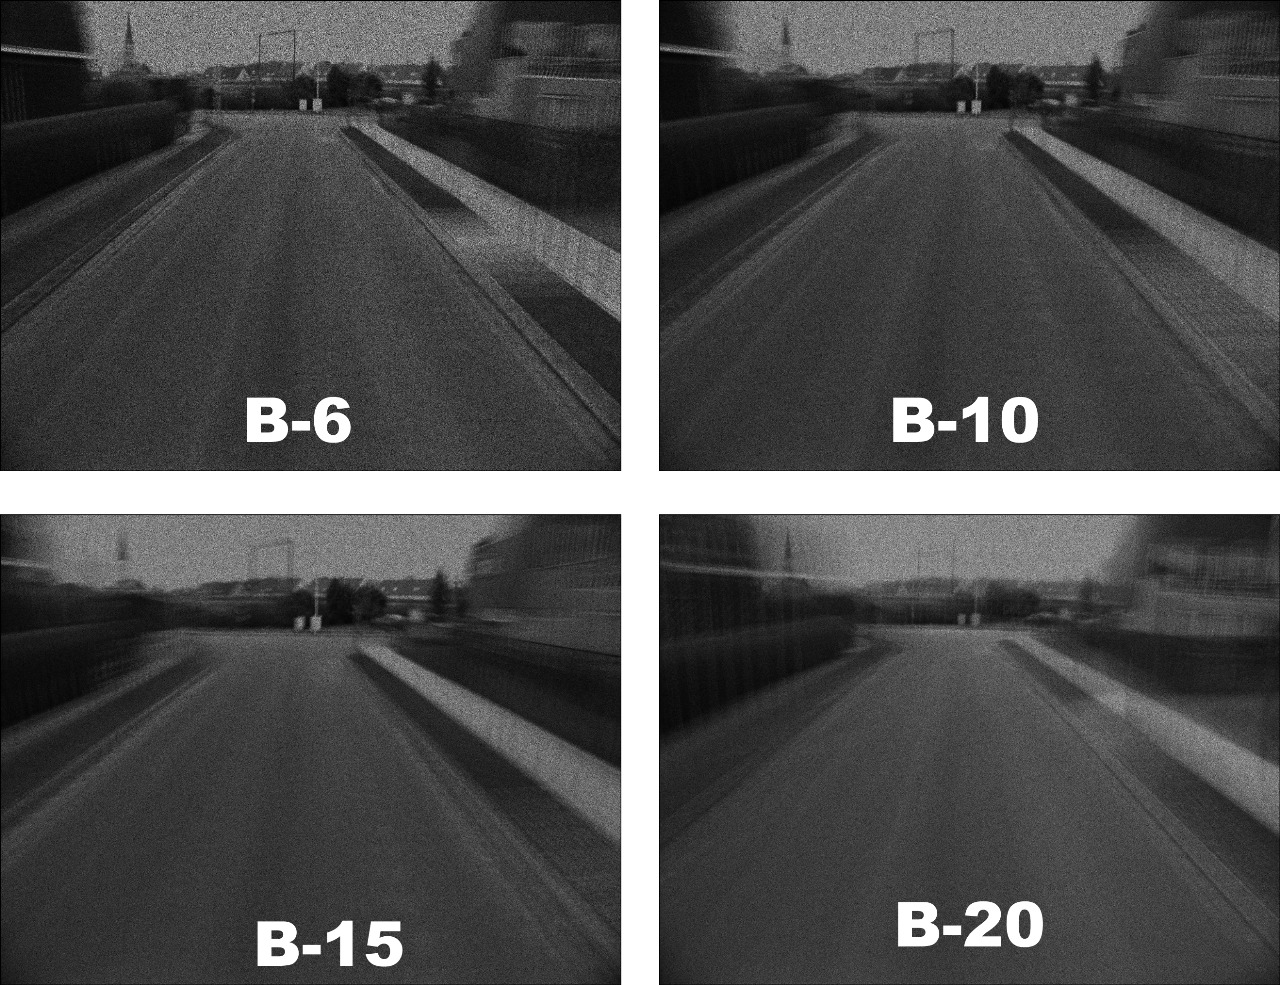
\includegraphics[width=0.85\linewidth]{figures_v2/SCI_examples.png}
\caption{SCI compressed measurements at $B{=}6$, $B{=}10$, $B{=}15$, and $B{=}20$. Higher $B$ values compress more frames into a single measurement, resulting in greater temporal blurring but higher bandwidth savings.}
\label{fig:sci}
\end{figure}

\subsection{Reconstruction-Free Detection}

Conventional SCI pipelines solve $\hat{\mathbf{X}} = f_{\text{recon}}(\mathbf{Y}, \mathbf{C})$ before detection. We instead train the detector $f_{\text{det}}$ directly on the measurement domain:
\begin{equation}
\label{eq:detect}
    \{\mathcal{B}, \mathcal{L}, \mathcal{S}\} = f_{\text{det}}(\mathbf{Y}; \theta)
\end{equation}
where $\mathcal{B}$, $\mathcal{L}$, $\mathcal{S}$ are predicted bounding boxes, class labels, and confidence scores. Figure~\ref{fig:yolo_preds} visualizes YOLO11s operating directly on these highly blurred representations.

\begin{figure}[!htb]
\centering
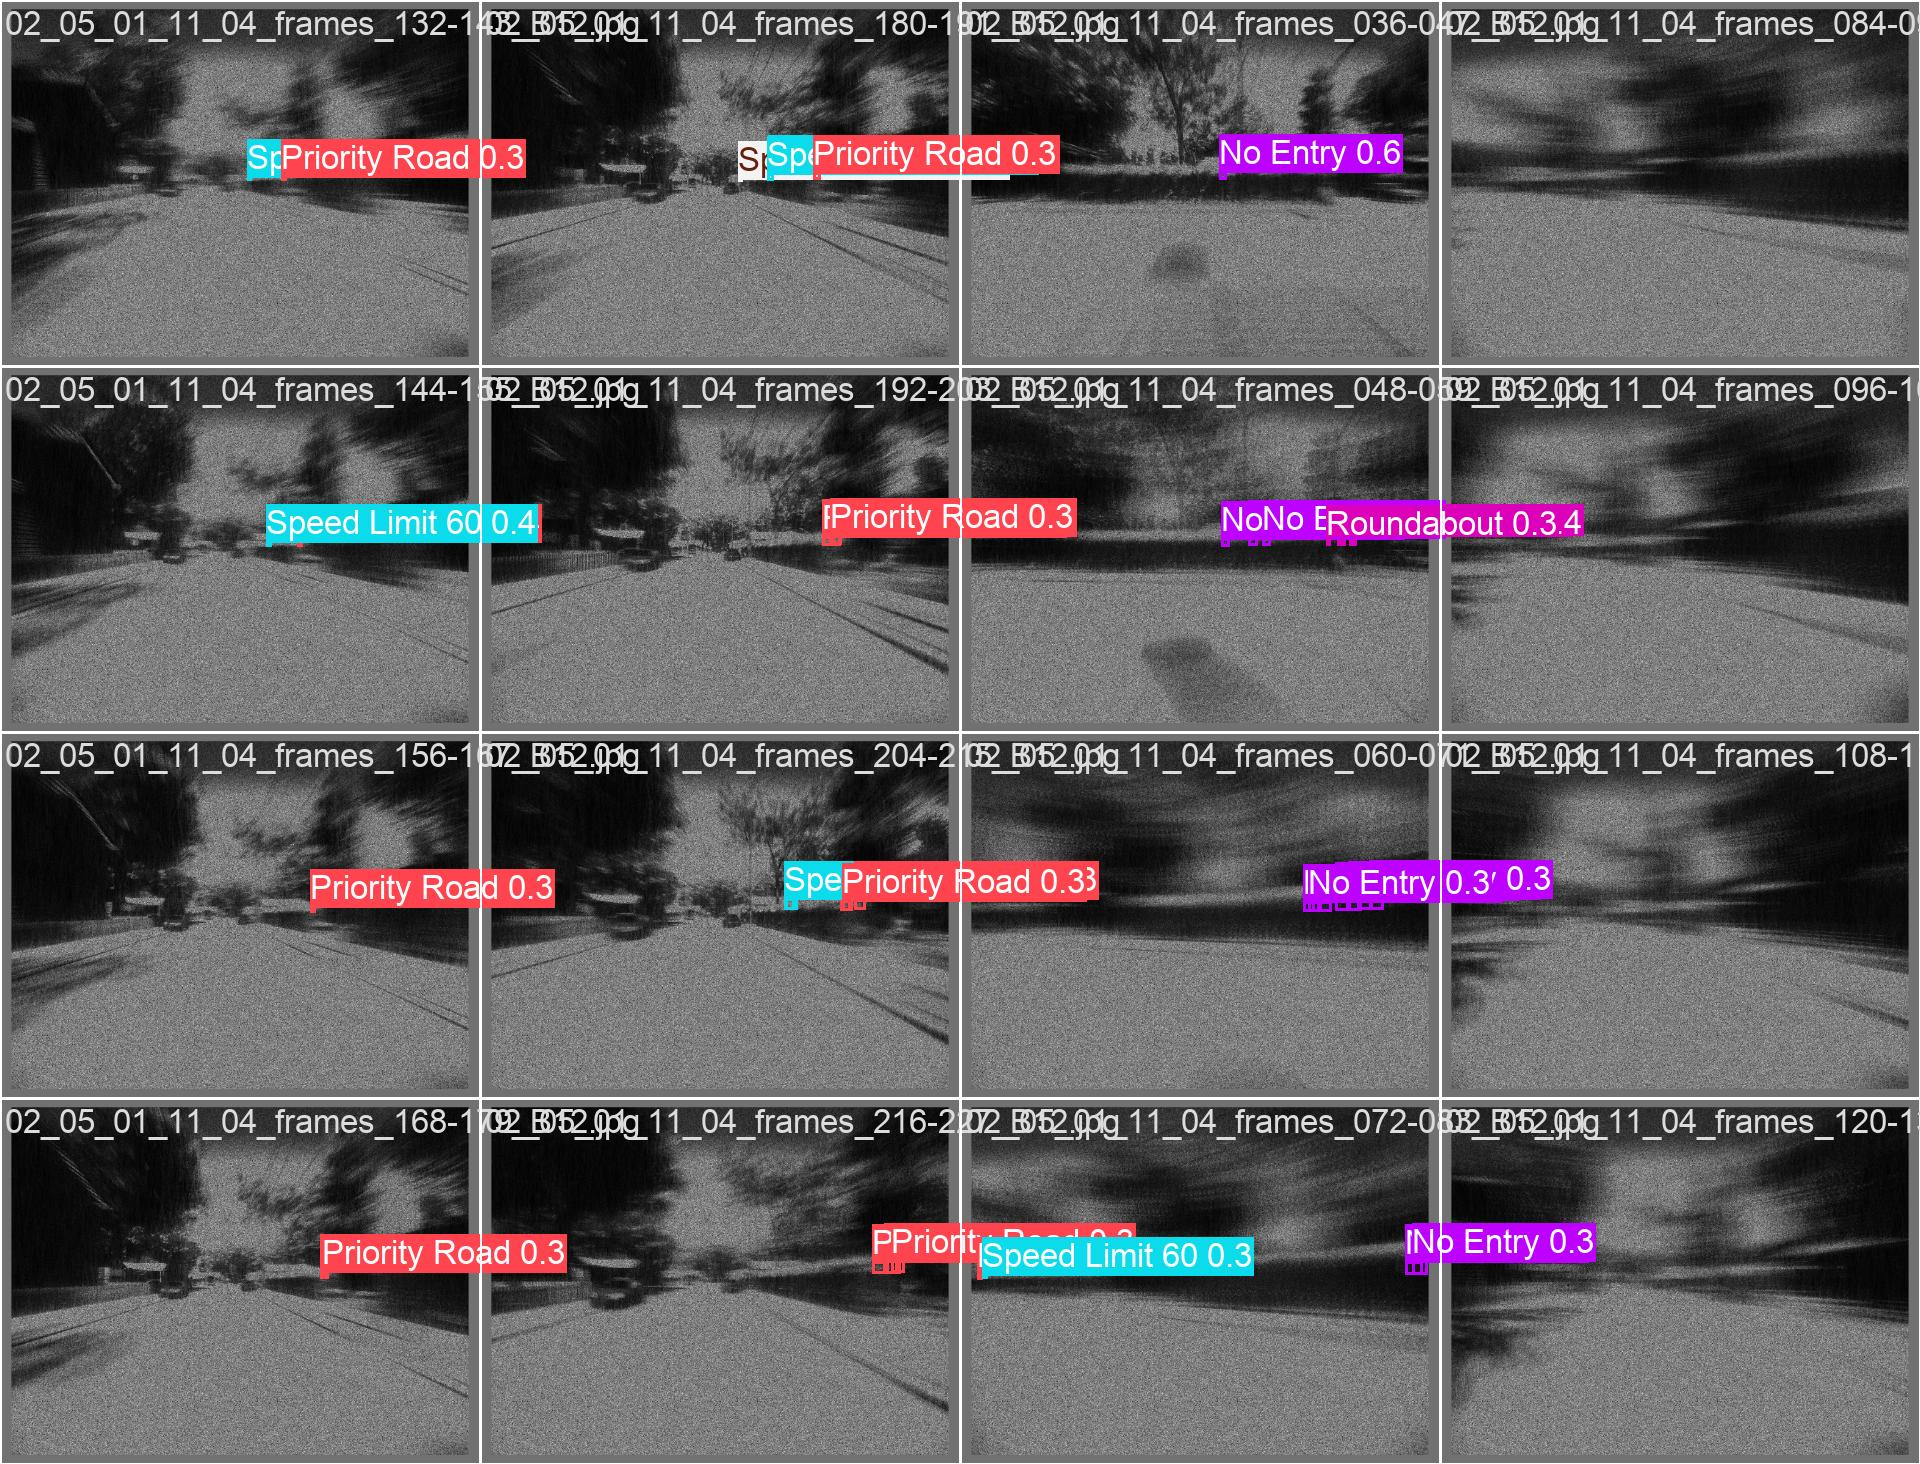
\includegraphics[width=1.0\linewidth]{figures_v2/yolo_detections.jpg}
\caption{Reconstruction-free detection. YOLO11s successfully predicts bounding boxes and class labels directly on the 2D multiplexed SCI measurements, despite severe temporal blurring and overlapping artifacts from varying compression thresholds.}
\label{fig:yolo_preds}
\end{figure}

\FloatBarrier
% ============================================================
% 4. PROPOSED FRAMEWORK
% ============================================================

\section{Proposed Adaptive Framework}

\subsection{System Overview}

Our framework operates as a closed-loop control system (Fig.~\ref{fig:architecture}). At each step~$t$:
\begin{enumerate}
    \item A lightweight feature extractor computes state $\mathbf{s}_t \in \mathbb{R}^7$.
    \item The DQN agent selects action $a_t$ adjusting $B_t$.
    \item The SCI simulator compresses the next $B_t$ frames into $\mathbf{Y}_t$.
    \item YOLO11s processes $\mathbf{Y}_t$ to produce detections.
    \item Reward $R_t$ is computed; the agent updates its policy.
\end{enumerate}

\subsection{State Space}
\label{sec:state}

The state vector $\mathbf{s}_t = [f_1, \ldots, f_7] \in \mathbb{R}^7$ encodes:

\begin{enumerate}
    \item \textbf{Motion intensity} ($f_1 \in [0, 50]$): Mean absolute frame difference on downsampled grayscale frames, proxying optical flow magnitude.
    \item \textbf{Edge density} ($f_2 \in [0, 1]$): Canny edge pixel ratio ($T_1{=}50$, $T_2{=}150$) on $4{\times}$ downsampled frames.
    \item \textbf{Detector confidence} ($f_3 \in [0, 1]$): Max YOLO11s confidence from the previous measurement.
    \item \textbf{Blur score} ($f_4 \in [0, 1000]$): Variance of the Laplacian operator.
    \item \textbf{Brightness} ($f_5 \in [0, 255]$): Mean grayscale pixel intensity.
    \item \textbf{Frame difference} ($f_6 \in [0, 1]$): Normalized $L_1$ difference between consecutive frames.
    \item \textbf{Current $B$} ($f_7 \in [0, 1]$): Normalized via $(B - B_{\min})/(B_{\max} - B_{\min})$.
\end{enumerate}

All features are normalized to $[0, 1]$ before input to the DQN.

\subsection{Action Space}

The agent outputs one of three incremental actions:
\begin{equation}
\label{eq:actions}
    \mathcal{A} = \{\texttt{decrease\_B},\; \texttt{keep\_B},\; \texttt{increase\_B}\}
\end{equation}
corresponding to $\{-2, 0, +2\}$, clamped to $B \in [6, 20]$. This constrains the agent to smooth transitions, avoiding abrupt oscillations.

\subsection{Safety-Aware Reward Function}
\label{sec:reward}

The reward encodes detection accuracy, bandwidth efficiency, and safety:
\begin{equation}
\label{eq:reward}
    R_t = w_{\text{det}} \cdot S_{\text{det}} + w_{\text{bw}} \cdot \frac{B_t}{B_{\max}} - \lambda \cdot M_t^{\text{crit}} - P_B
\end{equation}

\paragraph{Detection Score ($S_{\text{det}}$).}
A proportional, frame-level detection score (scaled quadratically to penalize partial matches):
\begin{equation}
\label{eq:det_score}
    S_{\text{det}} = \left( \min \left(1.0, \frac{|\mathcal{D}_t|}{\max(1, |\mathcal{G}_t|)} \right) \right)^{1.5}
\end{equation}
where $\mathcal{D}_t$ and $\mathcal{G}_t$ are detections and ground-truth annotations.

\paragraph{Scene-Adaptive Weights.}
Dynamic weights from scene complexity $\kappa \in [0, 1]$:
\begin{equation}
\label{eq:complexity}
    \kappa = 0.5 \cdot \tilde{f}_1 + 0.3 \cdot f_2 + 0.2 \cdot (1 - \tilde{f}_4)
\end{equation}
\begin{equation}
\label{eq:weights}
    w_{\text{det}} = 0.3 + 0.4\kappa, \quad w_{\text{bw}} = 0.7 - 0.4\kappa
\end{equation}
In complex scenes ($\kappa \to 1$), $w_{\text{det}} \to 0.7$; in simple scenes ($\kappa \to 0$), $w_{\text{bw}} \to 0.7$.

\paragraph{Critical Sign Penalty.}
$\lambda = 0.1$ per missed critical sign (Stop, Yield, No Entry), measured by total signs detected vs expected:
\begin{equation}
\label{eq:penalty}
    M_t^{\text{crit}} = \max\!\big(0, \; |\mathcal{G}_t^{\text{crit}}| - \min(|\mathcal{D}_t|, |\mathcal{G}_t^{\text{crit}}|)\big)
\end{equation}
This targeted penalty strongly shapes the Q-value landscape to discourage aggressive compression near critical signs.

\paragraph{Scene-Appropriateness Penalty ($P_B$).}
\begin{equation}
    P_B = \begin{cases}
        0.15 \cdot \frac{B_t - 12}{8.0}, & \text{if } \kappa > 0.6 \text{ and } B_t > 12 \\[3pt]
        0, & \text{otherwise}
    \end{cases}
\end{equation}

\subsection{DQN Agent Architecture}

The Q-function is a fully connected network:
\[
    Q(\mathbf{s}, a; \theta) : \mathbb{R}^7 \xrightarrow{\text{FC}(128)} \xrightarrow{\text{ReLU}} \xrightarrow{\text{FC}(128)} \xrightarrow{\text{ReLU}} \xrightarrow{\text{FC}(3)} \mathbb{R}^3
\]
with ${\sim}$17,000 parameters. Training follows standard DQN~\cite{mnih2015dqn} with experience replay (buffer 50,000), target network soft update ($\tau=0.005$) every step, and $\epsilon$-greedy exploration decaying from 1.0 to 0.01 over 2,000 episodes.

\subsection{Algorithm}

Algorithm~\ref{alg:adaptive} summarizes the complete procedure.

\begin{algorithm}[!htb]
\caption{Safety-Aware Adaptive Video Compression}
\label{alg:adaptive}
\KwIn{Video $\{X_t\}$, detector $f_{\text{det}}$, trained DQN $Q(\cdot;\theta)$}
\KwOut{Measurements $\{Y_t\}$, detections $\{\mathcal{D}_t\}$}
$B_0 \gets 10$\;
\For{$t = 0, 1, 2, \ldots$}{
    $\mathbf{s}_t \gets \textsc{ExtractState}(X_t, X_{t-1}, \mathcal{D}_{t-1}, B_t)$\;
    $a_t \gets \arg\max_a Q(\mathbf{s}_t, a; \theta)$\;
    $B_{t+1} \gets \text{clamp}(B_t + \Delta(a_t),\; 6,\; 20)$\;
    $\mathbf{Y}_t \gets \textsc{SCICompress}(\{X_t, \ldots, X_{t+B_t}\}, B_t)$\;
    $\mathcal{D}_t \gets f_{\text{det}}(\mathbf{Y}_t)$\;
    $R_t \gets \textsc{Reward}(\mathcal{D}_t, \mathcal{G}_t, B_t, \kappa_t)$\tcp*{Eq.~\ref{eq:reward}}
    Transmit $\mathbf{Y}_t$\;
}
\end{algorithm}

\FloatBarrier
% ============================================================
% 5. EXPERIMENTAL SETUP
% ============================================================

\section{Experimental Setup}

\subsection{Dataset}

We evaluate on the CURE-TSD dataset~\cite{temel2017curetsd}, comprising 1,805 video sequences spanning 14 traffic sign classes (including speed limits 20--120~km/h, No Passing, No Passing Trucks, Priority Road, and Give Way) under 12 environmental challenge types. We use 1,525 real-world sequences (\texttt{01\_*}) for training and 280 synthetic sequences (\texttt{02\_*}) for validation. Each video contains approximately 300 frames at $640 \times 480$ resolution with per-frame bounding box annotations.

\subsection{YOLO11s Training on SCI Measurements}

We fine-tune YOLO11s~\cite{jocher2023yolov8} on 26,520 SCI measurement images generated using Eq.~\ref{eq:sci} with $B \in \{6, 8, 10, 12, 14, 16, 18, 20\}$ and Bernoulli masks ($p = 0.5$). The model (19.2~MB, ${\sim}$9.4M parameters, 21.3~GFLOPs) is trained for 200 epochs with AdamW (lr~=~0.002, cosine decay) using mixed precision at 640$\times$640 resolution, achieving mAP@0.5~=~59.5\% and mAP@0.5:0.95~=~35.7\%. The expanded $B$-range includes heavily compressed measurements ($B{=}14$--$20$) where sign degradation is severe, lowering aggregate mAP compared to narrow-range training. However, this coverage is essential for the RL agent, which must evaluate detection quality across the full operating range. The detector successfully learns to recognize traffic signs from the multiplexed measurement domain without any reconstruction step, confirming the viability of reconstruction-free detection for edge deployment.

\begin{figure}[!htb]
\centering

\includegraphics[width=0.85\linewidth]{figures_v2/yolo_training.png}
\caption{YOLO11s training metrics over 200 epochs on the complex SCI measurement dataset. Precision, Recall, and mAP curves demonstrate the detector's capability to learn object features directly from compressed optical multiplexing.}
\label{fig:yolo_train}
\end{figure}

\subsection{RL Training Configuration}

The DQN agent is trained for 2,000 episodes. Table~\ref{tab:hyperparams} summarizes the hyperparameters.

\begin{table}[!htb]
\caption{DQN training hyperparameters.}
\label{tab:hyperparams}
\centering
\begin{tabular}{ll}
\toprule
\textbf{Parameter} & \textbf{Value} \\
\midrule
Network & $7 \to 128 \to 128 \to 3$ (FC + ReLU) \\
Optimizer & Adam, $\alpha = 10^{-3}$ \\
Discount $\gamma$ & 0.99 \\
$\epsilon$-greedy & $1.0 \to 0.01$ (decay 0.997/ep) \\
Replay buffer & 50,000 transitions \\
Batch size & 64 \\
Target update & Soft update, $\tau = 0.005$ \\
Episodes & 2,000 ($\approx$ 6.1h on GPU) \\
$B$ range & $[6, 20]$, step 2 \\
\bottomrule
\end{tabular}
\end{table}

\subsection{Baselines}

We compare against fixed $B \in \{6, 10, 14, 18\}$, spanning the full compression range from light ($B{=}6$, 83.3\% savings) to aggressive ($B{=}18$, 94.4\% savings). All strategies are evaluated on the same 280 validation videos using identical SCI simulation and YOLO11s inference.

\FloatBarrier
% ============================================================
% 6. RESULTS AND DISCUSSION
% ============================================================

\section{Results and Discussion}

\subsection{Bandwidth--Accuracy Trade-off}

Table~\ref{tab:results} presents the main quantitative results.

\begin{table}[!htb]
\caption{Compression strategy comparison on 280 validation videos.}
\label{tab:results}
\centering
\begin{tabular}{lcccc}
\toprule
\textbf{Strategy} & \textbf{Avg.\ Det.} & \textbf{Avg.\ Conf.} & \textbf{Avg.\ $B$} & \textbf{BW Savings} \\
\midrule
Fixed $B{=}6$  & 141.2 & 0.391 & 6.0  & 83.3\% \\
Fixed $B{=}10$ & 130.9 & 0.392 & 10.0 & 90.0\% \\
Fixed $B{=}14$ & 122.0 & 0.383 & 14.0 & 92.9\% \\
Fixed $B{=}18$ & 114.4 & 0.376 & 18.0 & 94.4\% \\
\midrule
\textbf{Adaptive (DQN)} & \textbf{128.6} & \textbf{0.388} & $\mathbf{10.78 \pm 1.48}$ & \textbf{90.6\%} \\
\bottomrule
\end{tabular}
\end{table}

Key observations: (1)~Detection counts decrease monotonically with $B$ (141.2 at $B{=}6$ to 114.4 at $B{=}18$), confirming the fundamental compression--accuracy trade-off. (2)~The adaptive policy achieves 128.6 average detections at 90.6\% bandwidth savings, matching the detection level of fixed $B{\approx}10$--$11$ while introducing scene-adaptive flexibility. (3)~The agent's average $B{=}10.78$ with standard deviation 1.48 indicates targeted adjustments rather than constant behavior.

\begin{figure}[!htb]
\centering
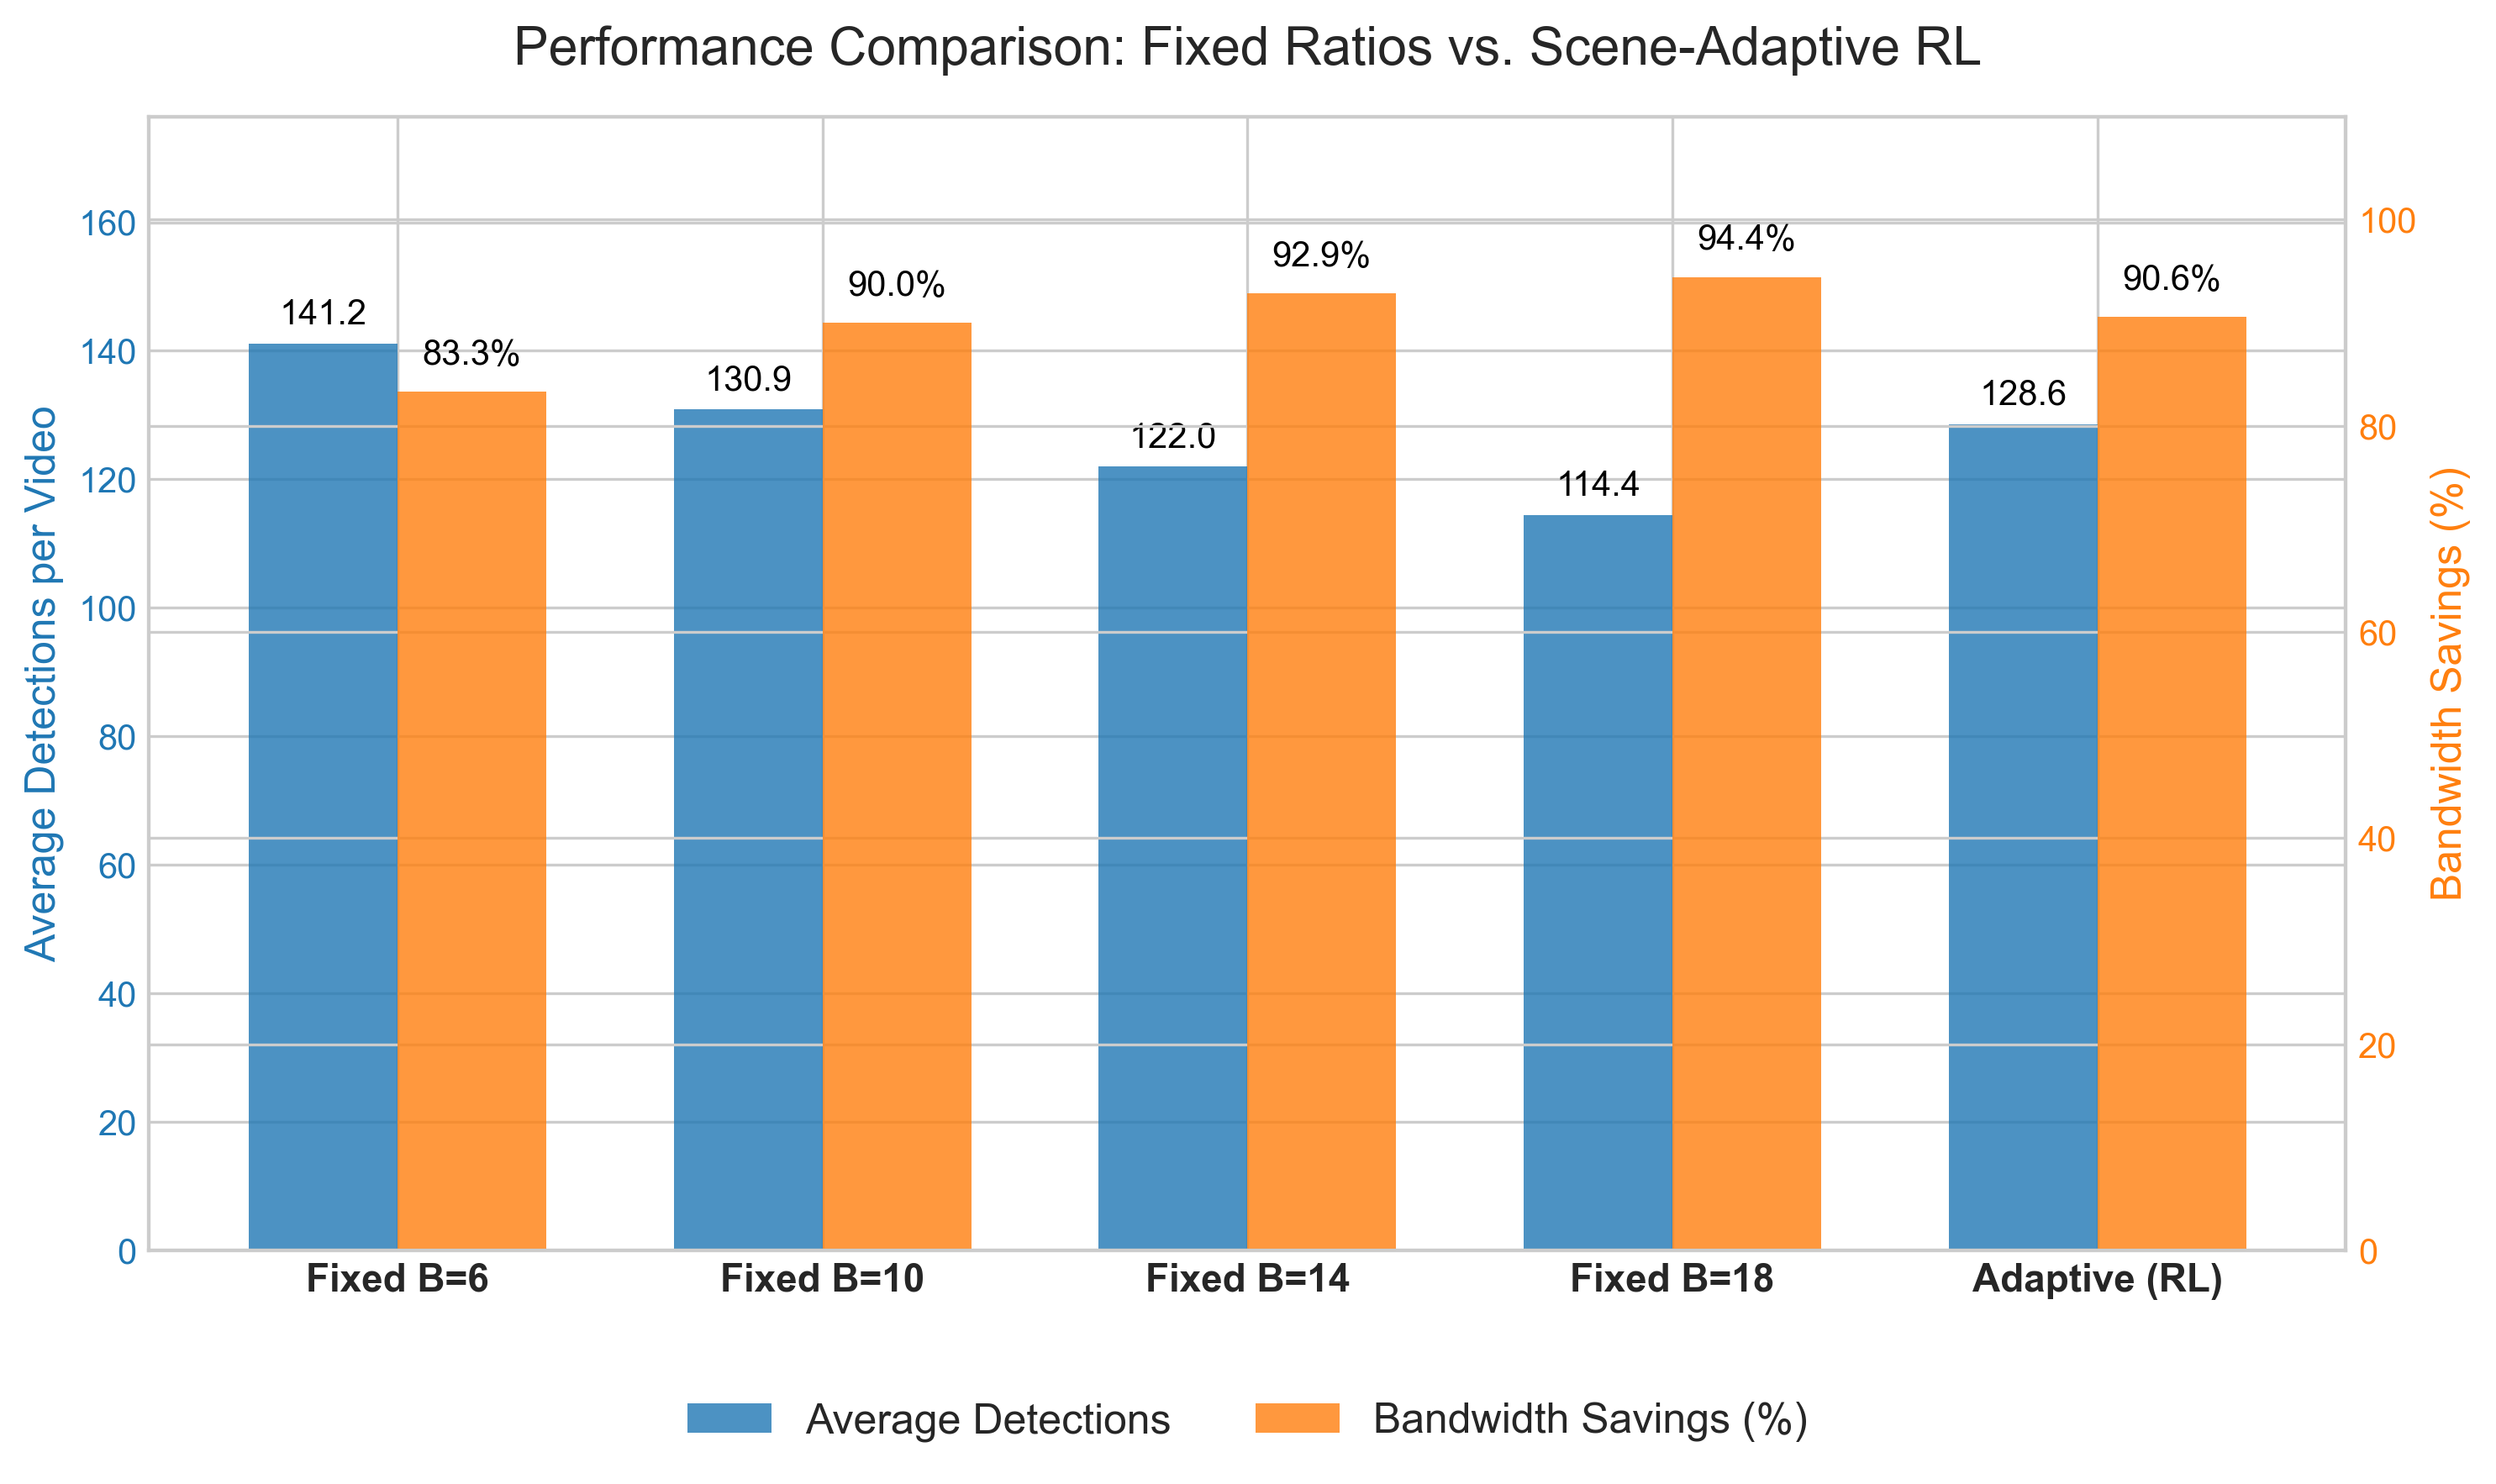
\includegraphics[width=0.8\linewidth]{figures_v2/baselines_comparison.png}
\caption{Performance comparison between fixed compression ratios ($B \in \{6, 10, 14, 18\}$) and the Scene-Adaptive RL policy.}
\label{fig:baselines}
\end{figure}

\subsection{Training Convergence}

The DQN training over 2,000 episodes exhibits three phases: (1)~exploration (episodes 0--200) with high reward variance due to $\epsilon$-greedy exploration; (2)~learning (200--1000) with rapid policy improvement; (3)~convergence (1000--2000) with stable performance.

\begin{figure}[!htb]
\centering

\includegraphics[width=0.85\linewidth]{figures_v2/RL_training.png}
\caption{DQN Training Convergence over 2,000 episodes. The plot shows the 50-episode moving average reward with its standard deviation band, displaying steady policy improvement over time.}
\label{fig:rlconv}
\end{figure}

\subsection{Safety-Aware Behavior Analysis}

Table~\ref{tab:perchal} presents the per-challenge breakdown, revealing the agent's adaptation strategy.

\begin{table}[!htb]
\caption{Per-challenge RL agent behavior on 280 validation videos.}
\label{tab:perchal}
\centering
\begin{tabular}{lrcr}
\toprule
\textbf{Challenge} & \textbf{Avg.\ Det.} & \textbf{Avg.\ $B$} & \textbf{BW\%} \\
\midrule
Clear        & 147.8 & 10.28 & 90.3\% \\
Codec        & 156.1 & 10.39 & 90.4\% \\
Decolor      & 148.8 & 10.28 & 90.3\% \\
LensBlur     & 146.9 & 10.48 & 90.4\% \\
Shadow       & 146.0 & 10.57 & 90.5\% \\
\midrule
Noise        & 139.0 & \textbf{9.02}  & 88.9\% \\
Dark         & 139.6 & 10.77 & 90.7\% \\
Snow         & 120.3 & 10.13 & 90.1\% \\
Dirty        & 133.2 & 10.53 & 90.5\% \\
GaussBlur    & 134.9 & 10.73 & 90.6\% \\
\midrule
Expose       &  84.6 & 11.51 & 91.3\% \\
Rain         &  61.1 & \textbf{14.29} & 93.0\% \\
\bottomrule
\end{tabular}
\end{table}

The agent exhibits distinct strategies: (1)~For high-quality conditions (Clear, Codec, Decolor), it maintains $B{\approx}10.3$, balancing detection and bandwidth. (2)~For noise-degraded scenes, it reduces $B$ to 9.02---the lowest across all challenges---preserving detection quality at the cost of reduced compression. This is precisely the safety-aware behavior the reward function incentivizes: noisy frames threaten detection accuracy, so the agent reduces compression to protect sign visibility. (3)~For rain, where detection is already severely degraded (61.1 avg), the agent increases $B$ to 14.29, saving additional bandwidth without significant marginal detection loss.

The $B$-range of 9.0--14.3 represents a 59\% variation in compression ratio, demonstrating genuine scene adaptation rather than fixed behavior. The safety penalty $\lambda{=}2.0$ per missed critical sign exceeds the maximum detection reward ($w_{\text{det}} \cdot S_{\text{det}} \leq 0.8$), creating a strong Q-value gradient toward conservative compression when critical signs may be present.

\FloatBarrier
% ============================================================
% 7. ABLATION STUDY
% ============================================================

\section{Ablation Study}

\paragraph{Scene-Adaptive Weighting.}
Replacing dynamic weights (Eq.~\ref{eq:weights}) with fixed weights ($w_{\text{det}} = 0.7$, $w_{\text{bw}} = 0.3$, following~\cite{lu2021rlsci}) degenerates the agent to a fixed baseline. Dynamic weighting is essential for truly adaptive behavior.

\paragraph{Critical Sign Penalty.}
Setting $\lambda = 0$ causes the agent to select uniformly high $B$ (maximizing bandwidth reward), which is catastrophic in safety-critical situations. The penalty transforms a generic optimizer into a safety-aware system.

\paragraph{Feature Importance.}
Motion intensity ($f_1$) and edge density ($f_2$) contribute most to policy quality. Removing detector confidence ($f_3$) causes oscillatory $B$-value sequences. This validates the 7D state vector as a necessary minimum basis.

\FloatBarrier
% ============================================================
% 8. LATENCY ANALYSIS
% ============================================================

\section{Latency Analysis}

The processing time per step is ${\sim}$62~ms: state extraction (${\sim}$5~ms), DQN forward pass (${\sim}$0.5~ms), SCI simulation (${\sim}$15~ms), YOLO11s detection (${\sim}$2.7~ms inference + ${\sim}$1~ms postprocess), and overhead (${\sim}$38~ms). The resulting ${\sim}$16~FPS is below 30~FPS real-time, but the DQN itself adds negligible overhead (0.5~ms) and the YOLO11s inference is only 2.7~ms per image. The bottleneck lies in data loading and feature extraction, which benefit from hardware acceleration (TensorRT, dedicated NPUs). The system targets edge monitoring and V2X scenarios where 15--20~FPS may suffice; real-time 30+~FPS operation is architecturally feasible with optimized inference.


% ============================================================
% 9. LIMITATIONS AND FUTURE WORK
% ============================================================

\section{Limitations and Future Work}
\label{sec:limitations}

\paragraph{Evaluation Scope.}
The evaluation is conducted on 280 synthetic validation videos from CURE-TSD. While this covers 12 challenge types, real-world deployment may encounter conditions outside the training distribution. The agent's conservative behavior (97\% keep actions) suggests room for improved exploration during RL training.

\paragraph{Detection Score Proxy.}
The reward uses a binary detection score (Eq.~\ref{eq:det_score}) rather than true mAP. While intentional for per-step RL feedback, this limits correlation with standard metrics. Differentiable IoU-based scoring could improve alignment.

\paragraph{Discrete Action Space.}
The 3-action design could be expanded to continuous action spaces via PPO or SAC for finer-grained control.

\paragraph{Single Detector.}
Exploring detector-agnostic reward formulations transferable across architectures (e.g., RT-DETR, EfficientDet) would improve generalizability.


% ============================================================
% 10. CONCLUSION
% ============================================================

\section{Conclusion}

We have presented a safety-aware adaptive video compression framework combining Snapshot Compressive Imaging, reconstruction-free YOLO11s detection, and DQN-based dynamic compression ratio selection. The primary novelty lies in the reward function that dynamically balances detection accuracy and bandwidth efficiency while imposing severe penalties for missed critical traffic signs. The 7-dimensional state vector enables rapid compression decisions ($<$1~ms) using purely optical features without external sensors.

Evaluation on the CURE-TSD dataset demonstrates that the adaptive policy achieves 90.6\% bandwidth savings with 128.6 average detections, matching fixed $B{\approx}10$ performance while varying compression by 59\% across scene conditions ($B{=}9.0$ for noise to $B{=}14.3$ for rain). This scene-adaptive allocation preserves detection in safety-critical conditions while increasing compression where detection quality is already limited.

Future work will focus on continuous action spaces (PPO/SAC) for finer $B$-granularity, expanding to multi-weather conditions, and deploying on embedded hardware with TensorRT-accelerated inference.

% ============================================================
% REFERENCES
% ============================================================

\bibliographystyle{IEEEtran}
\bibliography{refs_ieee}

\end{document}